% Kota Miura (miura at embl.de)
% BioImage Data Analysis Textbook 

\documentclass[11pt,a4paper,oneside]{report}
% Palatino for rm and math | Helvetica for ss | Courier for tt
\usepackage{mathpazo} % math & rm
\linespread{1.05}        % Palatino needs more leading (space between lines)
\usepackage[scaled]{helvet} % ss
\usepackage{courier} % tt

\normalfont
\usepackage[T1]{fontenc}
\usepackage[footnotesize]{caption}


\linespread{1.05}         % Palatino needs more leading (space between lines)

% space between paragraphs
\parskip 7.2pt

%making 1.5 spaced lines
\usepackage{setspace}
\onehalfspacing

% background shading
\usepackage{framed}

\usepackage{pdfsync}

% indent
\setlength{\parindent}{0in} % avoids indent at the beginning of paragraph


%\usepackage{url} % omitted, as this will just show url in different font
\usepackage[pdftex]{graphicx}

% equations
\usepackage{amsmath}
\usepackage{amssymb,amsfonts,textcomp}


%% Color definitions
\usepackage{color}
\definecolor{gray09}{rgb}{0.9,0.9,0.9}  %background for codes
\definecolor{red}{rgb}{1,0,0}
\definecolor{blue}{rgb}{0,0,1}
\definecolor{lightblue}{rgb}{0,0.8,1}
\definecolor{Dark}{gray}{.2}
\definecolor{Medium}{gray}{.6}
\definecolor{Light}{gray}{.8}
\definecolor{shadecolor}{rgb}{0.9, 0.9, 1}


%% enable using eps figure.
\usepackage{epstopdf}

%% Citations. 
%% Natbib is a popular style for formatting references.
\usepackage{natbib}
%% bibpunct sets the punctuation used for formatting citations.
\bibpunct{(}{)}{;}{a}{,}{,}

\usepackage{hyperref}
\hypersetup{colorlinks=true, 
	citecolor=blue, 
	linkcolor=black, 
	urlcolor=black}

% PDF linking
\usepackage{pdfpages}

%%%%%%%% Table Formattting %%%%%%%%%

\usepackage{supertabular}
\usepackage{array}
\usepackage{supertabular}
\usepackage{hhline}

%%%%%%%% Figure matters %%%%%%%%%%%

\usepackage{float}
\usepackage{subfig}
%\usepackage{caption}

%%%%%%%% Header and Footer %%%%%%%%
\usepackage{fancyhdr}
\setlength{\headheight}{15.2pt}
%\pagestyle{fancy}
\pagestyle{fancyplain}
\renewcommand{\chaptermark}[1]{\markboth{#1}{}}
\renewcommand{\sectionmark}[1]{\markright{\thesection\ #1}{}}
 
\lhead{\fancyplain{}{\textit{EMBL BIAS 2013}}}
\chead{}
\rhead{\fancyplain{}{\textit{\rightmark}}}
\lfoot{}
\cfoot{\fancyplain{}{\thepage}}
\rfoot{}


%%%%%%%% Custom Environments %%%%%%%%

%% a block for excercies
\newenvironment{indentexercise}[1]%
{{\setlength{\leftmargin}{2em}}%
\textbf{Exercise \thesubsection-#1}%
\begin{list}{}% 
	\item%
}
{\end{list}}

%% Indenting for ImageJ commands in a single line. 
\newenvironment{indentFiji}%
{\begin{list}{}%
         {\setlength{\leftmargin}{1em}}%
         \item[]%
}
{\end{list}}

%% indenting for what ever command in a single line. 
\newenvironment{indentCom}%
{\begin{list}{}%
         {\setlength{\leftmargin}{1em}}%
         \item[]%
}
{\end{list}}

%%% command for imageJ menu tree, in-line
\newcommand{\ijmenu}[1]{\texttt{\small#1}}

%%% command for inline command
\newcommand{\ilcom}[1]{\texttt{\small#1}}

%%% a quick command for making tab space
 \newcommand{\tab}{\hspace*{3em}}

%%% a quick command for horizontal line. 
\newcommand{\HRule}{\rule{\linewidth}{0.5mm}}

%% textcomp provides extra control sequences for accessing text symbols:
\usepackage{textcomp}
\newcommand*{\micro}{\textmu}
%% Here, we define the \micro command to print a text "mu".
%% "\newcommand" returns an error if "\micro" is already defined.


%%%%%%%%  Source Code Matters %%%%%%%%

% packge for codes
\usepackage{listings}
%\usepackage{listingsutf8}
\lstset{ %
%language=Octave,                % could choose the language of the code, but we go for black and white, no syntax highlighting defined. 
%basicstyle=\footnotesize,       % the size of the fonts that are used for the code
basicstyle=\small\ttfamily, % same as above, but use typewriter
numbers=left,                   % where to put the line-numbers
numberstyle=\footnotesize,      % the size of the fonts that are used for the line-numbers
stepnumber=1,                   % the step between two line-numbers. If it's 1 each line 
                                % will be numbered
numbersep=5pt,                  % how far the line-numbers are from the code
backgroundcolor=\color{gray09},  % choose the background color. You must add \usepackage{color}
keywordstyle=\color{red}, 	%added
showspaces=false,               % show spaces adding particular underscores
showstringspaces=false,         % underline spaces within strings
showtabs=false,                 % show tabs within strings adding particular underscores
%frame=single,                   % adds a frame around the code
%frame=trBL,
tabsize=2,                      % sets default tabsize to 2 spaces
captionpos=b,                   % sets the caption-position to bottom
breaklines=true,                % sets automatic line breaking
%breakatwhitespace=false,        % sets if automatic breaks should only happen at whitespace
title=\lstname,                 % show the filename of files included with \lstinputlisting;
                                % also try caption instead of title
escapeinside={\%*}{*)},         % if you want to add a comment within your code
morekeywords={*,...},            % if you want to add more keywords to the set
morecomment=[l]{//},
morecomment=[s]{/*}{*/},
morestring=[b]",
%aboveskip={7.2pt}	%supposed to be the space above llisting but dows not work. 
%belowskip={7.2pt}
}


%%%%%%%% title page matters %%%%%%%%  
% http://sunsite.bilkent.edu.tr/pub/tex/ctan/info/latex-samples/titlepages.pdf

%%%% Change title and the author. 
\newcommand*{\titleTH}{\begingroup% T&H Typography
\raggedleft
\HRule\\
\vspace*{\baselineskip}
{\Large Kota Miura}\\[0.167\textheight]

{\bfseries EMBL BioImage Data Analysis 2013}\\[\baselineskip]
{\textcolor{Medium}{\Huge ImageJ Macro Language}}\\[\baselineskip]
{\small May, 2013}\par
\vfill

%{\Large Centre for Molecular \& Cellular Imaging\\EMBL Heidelberg\\\plogo}\par
{\Large EMBL Heidelberg}\par
%\includegraphics[width=0.15\textwidth]{fig/rgb_logo_2006_win.eps} 
%\includegraphics[width=0.07\textwidth]{fig/Icon30pedge.jpg}\\[1cm] 
\vspace*{3\baselineskip}
\HRule\\
\endgroup}


%%%%%%%%%%%%%%%%%%%%%%%%%%%%%%%%%%%%%%%%%%%%%%%%%%%%%%%%%%%%%%%%%%%%%%%%%%%

\begin{document}

\date{\today}

\pagestyle{empty}
\titleTH
\clearpage
\pagestyle{fancyplain}

\begingroup
\hypersetup{linkcolor=black}
\tableofcontents
\endgroup

\clearpage

%%%% The chapter numer should be the numbering of the project  %%%% 
\setcounter{chapter}{2}

%%%% Insert the file name of the content %%%% 

\section{Aim}

Learn the basics of how to automate image processing and analysis using ImageJ macro language. We write macro for an easier life: less clicking and less repetitive workloads in BioImage Data Analysis. After quickly going through the syntax, we try writing a macro that measures intensity changes in the nucleus periphery over time. 

\section{Introduction}

To customize functions in ImageJ, one typical way is to write a Java plugin that directly accesses the application interface of ImageJ. This is a powerful method for customizing your own tool but in many cases is a bit too much for small tasks we often encounter in biological research. Compared to the Java programming, ImageJ macro is much easier for quickly solving problems. A typical usage is to automate repetitive tasks with hundreds of times of mouse clicking. By writing a macro, we could save such exhausting job to an execution of a macro file. As ImageJ macro functions are directly mirroring the GUI menu items, one could intuitively learn writing one's own macro even without much experiences in programming. 

Another important merit of writing a macro is its documentation aspect: as the processing becomes complex, we easily forget the steps and details of the procedures and the values of parameters that were used for that task. Even if your job is not a repetitive one, a macro written for a task becomes a valuable record of what was done to the image.  

In this short course, we will first start out with the basics of macro programming. We learn to handle variables, strings, looping and conditions and arrays. We then try writing a macro that processes two-channel image to segment nucleus in histone channel and use that information to measure the intensity changes in the second channel . Figure \ref{fig:strategy} shows two images that we analyze. If you compare these two images, you might realize that the green signal at the periphery of nucleus (red) is stronger in the second image. We will to quantify this difference.  

\begin{figure}[htbp]
 \centering
 \subfloat[Time point 1]{\label{fig:NucTimePoint1}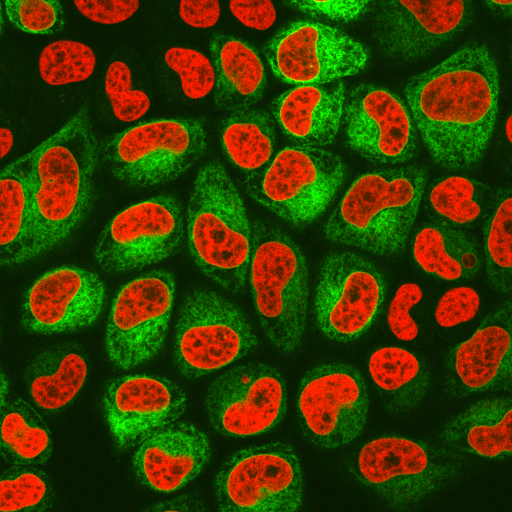
\includegraphics[width = 0.45\textwidth]{fig/NPC_T01.png}} 
 \quad
 \subfloat[Time point 15]{\label{fig:NucTimePoint15}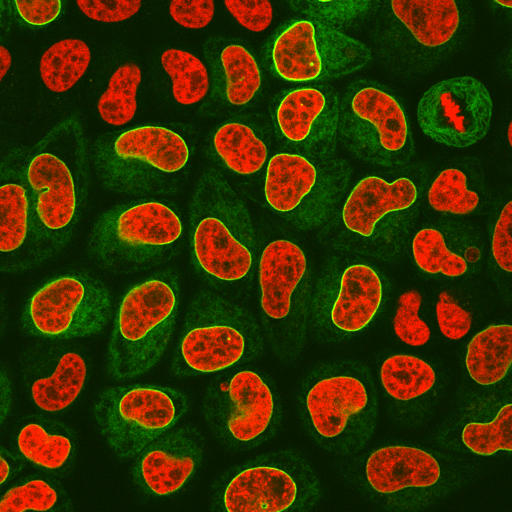
\includegraphics[width = 0.45\textwidth]{fig/NPC_T15.png}} \\
 \caption{NPC localization difference at two time points: More NPC in nucleus periphery. }
 \label{fig:NucMeasure}
\end{figure}

\subsection{Other ways to Customize ImageJ}

This and the next section explain general capability of extending ImageJ by programming and comparison with ImageJ macro, so if you are not interested in programming other than ImageJ macro, you could skip these sections and jump to the \ref{sec:tools}.  

In addition to Macro programming, ImageJ has plugin-writing capability.  This enables one to add new functions to ImageJ by coding in Java programming language. 
This capability affords almost infinite possibility to process and analyze images; 
you could create any kind of processing / analysis functions you could imagine. 
Compared to plugins, ImageJ Macro language has some limitations: 

\begin{enumerate}
\item If you need to process large images or stacks with many steps, 
you might recognize that it is slow. 
Some benchmarks indicates that a plugin would be about 40 times faster than Macro. 

\item Macro cannot be used as a library
\footnote{It is possible to write a macro in a library fashion and use it from another macro, 
but this is not as robust and as clear as it is in java, which is a language designed to be so.}. 
In Java, once a class is written, this could be used later again from another class . 

\item Macro is not efficient in implementing real-time interactive input 
during when the macro function is executed; 
\textit{e.g.} If you want to design a program that requires real-time user input 
to select a ROI interactively.  
Macro could only do such interactive tasks by closely related macro set with each macro doing each step of interaction. 

\item Macro is tightly coupled to GUI (Image Window), so that when you want to process images without showing them on desktop, macros are not really an optimal solution.  
\end{enumerate}

If you become unsatisfied with these limitations, 
learning more complicated but more flexible java plugin development is recommended. 


\subsection{Comparison with Other scripting languages}

Besides ImageJ macro, there are several scripting languages that
could be used for programming. Bare ImageJ supports Javascript (Rhino).
In the Fiji distribution, you could use the following languages:

\begin{itemize}
 \item Javascript
 \item BeanShell
 \item Jython (Java implemented Python)
 \item JRuby (Java implemented Ruby)
 \item Clojure
 \end{itemize}

If you set up environment by yourself, you could also use other languages such as Scala and Groovy. 
Compared to the ImageJ macro language, all these languages are more general and widely used. 

Merits of using the ImageJ Macro compared to these scripting languages are: 
\begin{itemize}
\item Easy to learn. 
ImageJ macro build-in functions are mirrors of ImageJ menu, so scripting is intuitive if you know ImageJ already. 
Macro recorder is a handy tool for finding out the macro function you need. 

\item You could have multiple macros in one file (called 'Macro-set"). 
This is useful for packaging complex processing tasks.

\item A significant hurdle for coding with general scripting languages is that one must know the 
\textbf{ImageJ Java API} well, meaning that you basically have to know 
fundamentals of Java programming language for using these scripting languages. 
\end{itemize}

Thus, ImageJ macro language is the easiest way to access the scripting
capability of ImageJ.

There are several disadvantages of ImageJ macro compared to other
scripting languages. First is its generality. Since others are based on major scripting languages, you do not need to learn a lot if you know one of them already. For example, if you know Python already, 
it should be easy for you to start writing codes in Jython. 

Second disadvantage is its extendability.
Codes you wrote could only be recycled by copy and pasting
\footnote{One could also use getArgument() and File related functions to pass
arguments from a macro file to the other, but ImageJ macro is not designed to
construct a library of functions.}.
With other scripting languages, one could write object-oriented programs 
and once you write them, the code could be used from other programs
\footnote{ Calling other Javascript file from another Javascript file had been difficult but became easily possible in the Fiji distribution from March 2012.}.

Lastly, although ImageJ Macro processes with a speed comparable to
Javascript and Jython, it is slow compared to Clojure and Scala. 


\section{Tools}
\label{sec:tools}

\begin{itemize}
    \item ImageJ (Fiji distribution).
    \begin{itemize}
        \item \url{http://fiji.sc}
	\item We use the Fiji distribution since it has ScriptEditor, a handy editor for writing macro. 
    \end{itemize}
    \item ImageJ Plugin: CourseModules\_.jar
      \begin{itemize}
        \item \url{http://cmci.embl.de/downloads/coursemodules}
        \item This plugin allows you to download sample image stack.
      \end{itemize}
\end{itemize}


\section{ImageJ Macro Basics}

\subsection{``Hello World!''}
We first try writing a simple macro that prints ''Hello World!'' in the log window of ImageJ. 
The Fiji distribution has a script editor with simple debugger function

\footnote{Debugger assists you to correct mistakes in the code. 
This is convenient when the code becomes long. 
Macro can be written in any text editor such as "Notepad" in Windows but of course 
there is no debugger function available in this case.}. 

To open the editor, select \ijmenu{[File -> New -> Script]} from the menu bar. 
It should look like \ref{fig_ScriptEditor}. 
In the script editor, you already see a blank text field where you could write a macro. The script editor has it's own menu, and to use ImageJ macro select \ijmenu{[Language -> ImageJ Macro]}. 

Later when you want to start writing another new macro, just generate a new tab by \ijmenu{[File > New]} and then select \ijmenu{[Language -> ImageJ Macro]} again.
 
Then write your first macro as shown below. 

\begin{quote}
\ilcom{print("Hello World!");}
\end{quote}

See the figure \ref{fig_ScriptEditor}. Don't ignore quotes, parenthesis and semi-colon!
Syntax high-lighter offers automatic coloring of ImageJ functions. 

\begin{figure}[hbtp]
\begin{center}
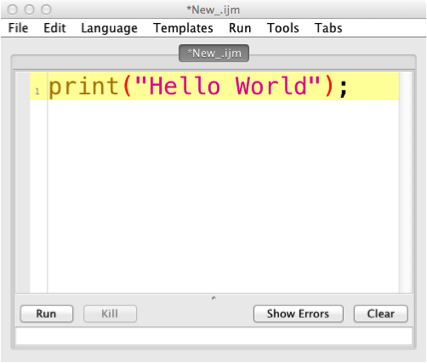
\includegraphics[scale=1.0]{fig/editor_helloworld_singleline.png}
\caption{Script Editor of the Fiji distribution} \label{fig_ScriptEditor}
\end{center}
\end{figure}

Then in the script editor at left bottom corner, there is a button labeled "Run". Clicking this, you will see that a log window is created (if it is already there, then will have a new line) printing "Hello World!" (Figure \ref{fig_HelloWorldLog}). Another way to run the macro is via Script Editor menu,  \ijmenu{[Run -> Run]} . You could use Ctrl-R (Windows) or Command-R (OSX) as well.  

\begin{figure}[hbtp]
\begin{center}
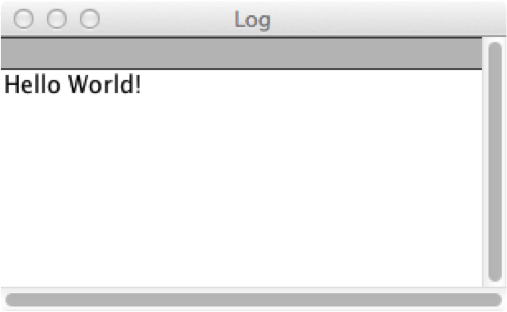
\includegraphics[scale=1.0]{fig/helloworld_logwindow.png}
\caption{Hello World Output} \label{fig_HelloWorldLog}
\end{center}
\end{figure}

\subsubsection{Anatomy of ``Hello World!''}

print() function orders ImageJ to print out the content within the parenthesis 
in the "Log" window. The text to be printed must be contained within the double quotes (""). 
The best reference for ImageJ macro functions is in the ImageJ web site
\footnote{\url{http://rsbweb.nih.gov/ij/developer/macro/functions.html}}. 
For example, you could find definition of print("") function in the web site as quoted in below:\\
%\item
\begin{indentCom}
%\begin{minipage}[c][18em][c]{0.85\textwidth}
\fbox{
\parbox[b][20em][c]{0.80\textwidth}{
\textbf{print(string)}\\
Outputs a string to the "Log" window. Numeric arguments are automatically converted to strings. 
The print() function accepts multiple arguments. For example, you can use print(x,y,width, height) 
instead of print(x+" "+y+" "+width+" "+height). 
If the first argument is a file handle returned by File.open(path), 
then the second is saved in the referred file (see SaveTextFileDemo).

Numeric expressions are automatically converted to strings using four decimal places, 
or use the \ilcom{d2s} function to specify the decimal places. 
For example, print(2/3) outputs "0.6667" but print(d2s(2/3,1)) outputs "0.7".
}
}
\end{indentCom}

If your machine is connected to the Internet, double clicking a function will automatically open web browser and guide you directly to the function help. From the menu the same could be done by \ijmenu{[Tools > Open Help for Macro Function]}.

So that was the basics of how to write and run a macro. Macro can be saved as a file.
In the editor, do \ijmenu{[File -> Save]}. Just save the file wherever you want in your file system . 

%\begin{indentexercise}{1cm}
\begin{indentexercise}{1}
\item Add another line \texttt{"print("\textbackslash{}\textbackslash{}Clear");"} 
after the first line (below, code 1.51. don't forget the semi-colon at the end!). 
\item \lstinputlisting{code/code01_51.ijm}
Then test also another macro when you insert the same function in the second line (code 1.76). 
What happened? Any difference in the behavior? 
\item \lstinputlisting{code/code01_76.ijm}
\end{indentexercise}

\begin{indentexercise}{2}
\item Try modifying the third line in code 1.51
and check that the modified text will be printed in the "Log" window. \\
\end{indentexercise}

\begin{indentexercise}{3}
\item Multiple macros can exist in a single file. We call this \textbf{"macro sets"}. To distinguish each macro, they each should have some name of the macro. For this each macro should start with a special word ``macro'' followed by the name of the macro, and then a pair of curly braces to encapsulate its macro functions. See the code below.  

\lstinputlisting{code/code01_8.ijm}

Modify the code you already wrote in the script editor to wrap it inside a macro bounds.  Then copy and paste the same under the first macro. 
The second macro should be modified to have a different name. In the example shown in fig.
\ref{fig_MacroSetInMenu}, the second macro is named "pirnt\_out2".
\begin{figure}[htbp]
\begin{center}
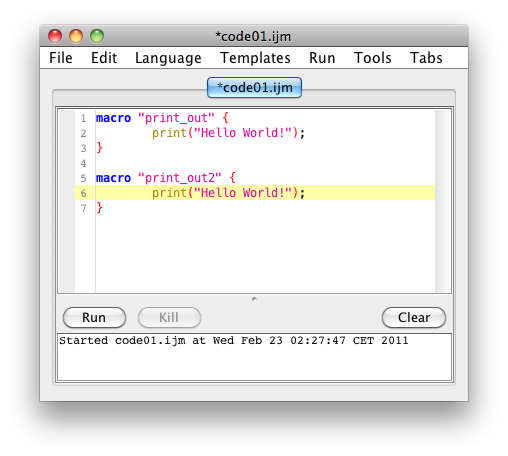
\includegraphics[scale=0.6]{fig/editor_MacroSet.png}
\caption{Macro Set} \label{fig_MacroSetInMenu}
\end{center}
\end{figure}
When macro is properly declared in this way, you could install the macro to have it as a menu item. To do so, in the editor menu select: 
\begin{indentFiji}
[Run -> Install Macro]).
\end{indentFiji}
In the main menu you should no be able to see the macro names under \ijmenu{[Plugins > Macros > ]}.

\begin{figure}[htbp]
\begin{center}
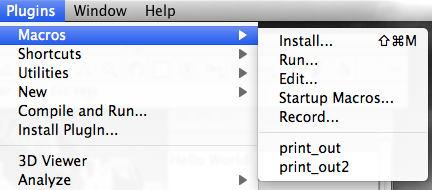
\includegraphics[scale=0.6]{fig/firstMacroSetInMenu.png}
\caption{Macro Now in ImageJ menu} \label{fig_MacroInMenu}
\end{center}
\end{figure}
\end{indentexercise}

\subsection{Variables and Strings}
Texts such as "Hello World!" can be represented by a variable 
\footnote{there is no declaration of types, such as number or string, in ImageJ macro.}.
Let's understand this by examining a short macro below.
\lstinputlisting{code/code02.ijm}

\ilcom{text} is a "String Variable" or simply a "String". 
ImageJ prepares a memory space for this variable, and you can change the content by re-defining the content. Two (or maybe more) variables could be used to construct another variable. 

\lstinputlisting{code/code03.ijm}

The above operation concatenates content of \ilcom{text2} to the content of \ilcom{text1} and produces a third variable \ilcom{text3} that holds the result of concatenation. 

\begin{indentexercise}{1}
\item Add more string variables and make a longer sentence.\\
\end{indentexercise}


It is also possible to substitute the variable content with numbers, such as\\
\begin{lstlisting}[numbers=none]
text = 256;
\end{lstlisting}
With this assignment, the variable is now a "numerical variable" or simply "variable". 
In other programming languages such as C or Java, difference between numbers and characters matters a lot. 
In ImageJ macro you do not have to care whether the variable is number or string,  but in some cases this may cause problem 
so it's better to just keep this difference in your mind. We will see an example of such confusion, 
and also a way to avoid the confusion. 

Test the following macro to see how the numerical variable works. 
\lstinputlisting{code/code04.ijm}
Did you get some results printed out? It should, but you should read the code carefully. 

You might have noticed a strange expression at line 8, in the way it assigns the variable txt. 
It starts with double quotation marks. \\
%\lstinputlisting[language=Java, linerange={8-8}, numbers=none]{code/code04.ijm}
\begin{lstlisting}[numbers=none]
txt= "" + a + "+" + b + "=" + c;
\end{lstlisting}
Seemingly this looks like meaningless. 
If you define txt without the first "useless" quotation marks, then it will be like\\
\begin{lstlisting}[numbers=none]
txt= a + "+"+ b + "=" + c;
\end{lstlisting}
Theoretically this should work also, 
since the double quotes does not have any content so it's presence should be meaningless. But if you try to run this what it seems to be straight-forward assignment, 
ImageJ returns an error message. 

\begin{figure}[htbp]
\begin{center}
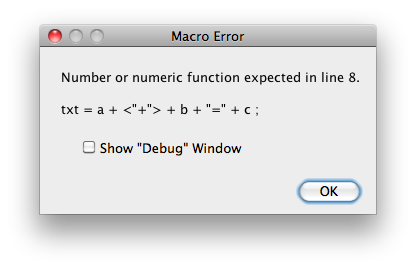
\includegraphics[scale=0.6]{fig/ErrorStringNumericFunction.png}
\caption{Error with Variable Assignment} \label{fig_ErrorVariable}
\end{center}
\end{figure}

This is because when ImageJ scans through the macro from top to bottom, line by line, 
it reaches the line for the assignment of the variable \ilcom{txt} and first sees the variable \ilcom{a} and interprets that \ilcom{txt} should be a numerical variable 
(or function), since \ilcom{a} is known to be a number as it was defined so in one of the lines above. Then ImageJ goes on interpreting rightward thinking that this is math. Then finding a "+" which surprisingly is a character
ImageJ cannot interpret string variable within a numerical function, so it returns an error message. The macro aborts.  

To overcome this problem, the programmer can tell ImageJ that 
\textit{txt} is a string function at the beginning of the assignment 
by putting a set of double quote. This tells the interpreter that this assignment is a string concatenation assignment and not a numerical assignment. 
ImageJ does handle numerical values within string function, 
so the line is interpreted without problem and prints out the result successfully.  

\begin{indentexercise}{2}
Modify the code 4, so that the calculation involves subtraction (-), multiplication (*) and division (/). 
\end{indentexercise}

\subsection{Recording ImageJ macro functions}
There are many functions in ImageJ as you could see them by exploring the menu. Almost all of these commands can be accessed by build-in macro functions\

{Some plugins are not macro-ready.}.

We will make a macro that creates a new image, add noise, blurs this image by Gaussian blurring, and then thresholding the image. To know required macro function there is a very convenient tool called \textbf{Command Recorder}. 
Do \ijmenu{[PlugIns -> Macros -> Record\ldots]}. A window like figure
\ref{fig_macroRecorderBlank} opens.

\begin{figure}[htbp]
\begin{center}
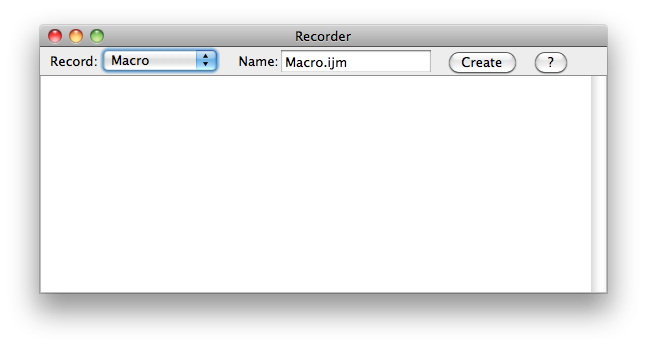
\includegraphics[scale=0.6]{fig/MacroRecorderBlank.png}
\caption{Macro Recorder} \label{fig_macroRecorderBlank}
\end{center}
\end{figure}

All the menu commands that you execute will be printed out as a history of macro functions in this window. For composing a macro using this recorder, we first do the processing manually from the menu as follows. 
\begin{itemize}
  \item Prepare a new image using \ijmenu{[File -> New]} command. Size of the image can be anything.
  \item Then do \ijmenu{[Process -> Noise -> Salt and Pepper]} (Fig.
  \ref{fig_SaltAndPepper}).
  \item \ijmenu{[Process -> Filters -> Gaussian Blur]} (use Sigma = 2.0).
  \item \ijmenu{[Image -> Adjust -> Threshold\ldots]}. Toggle the slider to make
  signals red. Check "Dark Background", then click "Apply".
\end{itemize}
 
\begin{figure}[htbp]
\begin{center}
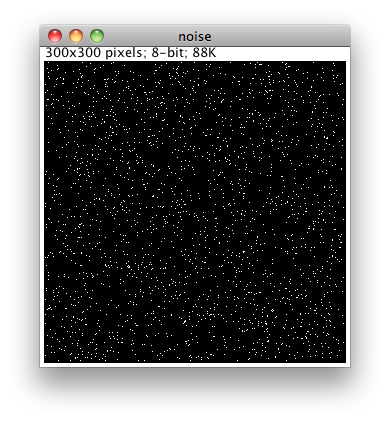
\includegraphics[scale=0.6]{fig/SaltandPepper300.png}
\caption{A demo image for Recording Macro} 
\label{fig_SaltAndPepper}
\end{center}
\end{figure}

Now, check the Command Recorder window. 
It should now look like Fig. \ref{fig_macroRecorderFilled}. 
Lines appeared after your operations are corresponding macro functions.

\begin{figure}[htbp]
\begin{center}
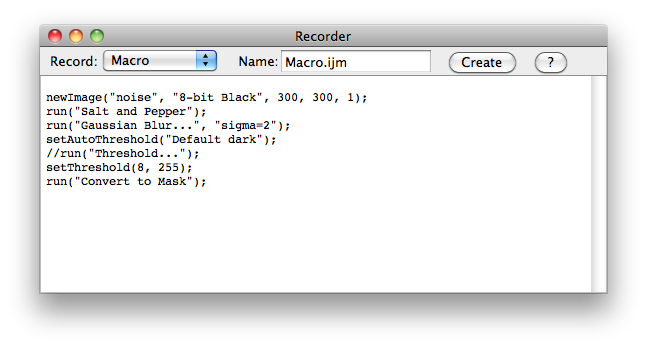
\includegraphics[scale=0.6]{fig/MacroRecorderFilled.png}
\caption{Macro Recorder after some lines Recorded} 
\label{fig_macroRecorderFilled}
\end{center}
\end{figure}

These texts generated in in the recorder can be used as it is in your macro.  You could copy and paste them\footnote{In case of OSX, you might probably need to click ``Create'' button to generate a duplicate of macro functions in a new script window. Then you could copy the macro functions from there.}. Compose a macro like below by copy and pasting the macro functions in the recorder.  Delete the lines that is commented out (lines that begins with "//" are lines that are skipped by the macro interpreter).
\lstinputlisting{code/code06_9.ijm}

Run the macro! \ldots I hope that you are amazed by now with the power of Macro
Recorder! Now, you could simple add a line at the top and bottom to package this in a named macro. This is optional in the current case, but it's always good to keep your macro like this since boundary of the macro becomes clear. 
 
\lstinputlisting{code/code07.ijm}

The second line in the above macro has a function \ilcom{newImage()}. This
function creates a new image. It has five arguments (in coding jargon, we say
there are "five arguments"). To know what these arguments are, 
the quickest way is to read the Build-In Macro Function page in ImageJ web site  
(the reference is attached to this manual so take a look).  
In case of newImage function, the description looks like this. 

\begin{indentCom}

\fbox{
\parbox[b][16em][c]{0.80\textwidth}{
\textbf{newImage}(title, type, width, height, depth)\\
Opens a new image or stack using the name title. 
The string type should contain "8-bit", "16-bit", "32-bit" or "RGB". 
In addition, it can contain "white", "black" or "ramp" (the default is "white"). 
As an example, use "16-bit ramp" to create a 16-bit image containing a grayscale ramp.  Width and height specify the width and height of the image in pixels.  Depth specifies the number of stack slices.
}}
\end{indentCom}
Using this information, you can modify the macro to change the size of the image.

\begin{indentexercise}{1}
Modify the code 7 and try changing the size of window to be created.
\end{indentexercise}

Another optional lines you could add to the macro are ``comments''. This does not affect the macro but adding some comment about what the macro does helps you to understand what the macro is doing when you open the file some time later. There are two ways to add comment. One is block comment. Texts bounded by \ilcom{ /*} and \ilcom{*/} will be ignored by interpreter. Another is line commnet. Texts in a line starting with double slash \ilcom{//} will be ignored by the interpreter. Below is an example of commenting code 07. 

\lstinputlisting{code/code07_1.ijm}

\subsection{Conditions and Loops}
In many cases, we want to iterate certain processing many times ("Loops": see middle in the figure \ref{fig_scriptscheme}), or we want to limit some of the process in the program only for certain situations ("Conditions": see right of the figure \ref{fig_scriptscheme}). In this section we learn how to include these loops and conditional behaviors into macro. 

\begin{figure}[htbp]
\begin{center}
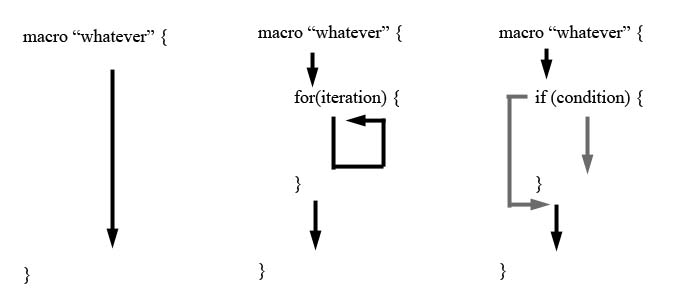
\includegraphics[scale=0.55]{fig/fig23_1_ScriptSchemes.png}
\caption{Schematic view of conditions and loops. Single line by line processing and macro with loops (middle) or with condition (right).} \label{fig_scriptscheme}
\end{center}
\end{figure}

\subsubsection{Loop: for-looping}
Here is a simple example macro using for-loop. Write the macro in your editor and run it. 
\lstinputlisting[morekeywords={*, for}]{code/code08_9.ijm}
%\lstinputlisting[morekeywords={*, for}]{code/code09.ijm}
The result should look like figure \ref{fig_whateverOut}.

%whatever x 5 figure
\begin{figure}[h!]
\begin{center}
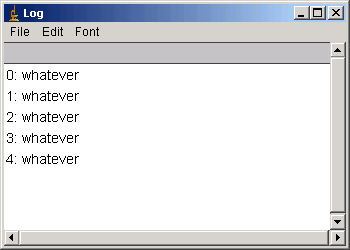
\includegraphics[scale=0.6]{fig/fig2311_whatever5.png}
\caption{Code 9 output in Log Window}
\label{fig_whateverOut}
\end{center}
\end{figure}

\begin{itemize}

\item Line 3 \ilcom{for( i = 0 ; i < 5 ; i+= 1)} sets the number of loops. 
Three parameters are required for "for" loop. The first parameter defines the variable used for the counting loop and its initial value (\ilcom{i = 0}). The second parameter sets the condition for exiting from the loop (\ilcom{i < 5}). Third parameter sets the step size of i, meaning that how much value is added per loop (\ilcom{i += 1}, could also be subtraction, multiplication, division e.g. \ilcom{i -= 1}). 
\item After this \ilcom{for(\ldots;\ldots;\ldots)} statement, there is a brace (\{) at the end of line 3 and the second one in the line 5. These curly braces tell ImageJ to loop macro functions in between so the function in line 4 will be iterated according to the parameters defined in the parenthesis of \ilcom{for}. Between braces, you could add more lines of macro functions as many as you want.  
\end{itemize}
So when the macro interpreter reaches line 3 and sees \ilcom{for(}, it starts looking inside the parenthesis and defines that the counting starts with 0 using a variable \ilcom{i}, and then line 4 is executed. The macro prints out "0 \ensuremath\colon whatever" using the content of \ilcom{i}, string \ilcom{\ensuremath\colon} and the string variable \ilcom{txt}. 
Then in line 5, interpreter sees the boundary \ilcom{\}} and goes back to line 3 and adds 1 to i (because of \ilcom{i+=1}). i = 1 then, so \ilcom{i<5} is true. The interpreter proceeds to line 4 and executes the macro function and prints out "1\ensuremath\colon whatever".  Such looping will continue until i = 5, since only by then \ilcom{i<5} is no longer true so interpreter exits from the for-loop. \\

\begin{indentexercise}{1}
(1) Change the first parameter in \ilcom{for(i=0;i<5;i+=1)} so that the macro prints out only 1 line. 

(2) Change the second parameter in \ilcom{for(i=0;i<5;i+=1)} so that the macro prints out 10 lines. 

(3) Change the third parameter in \ilcom{for(i=0;i<5;i+=1)} so that the macro prints out 10 lines. 
\end{indentexercise}

\subsection{Stack Analysis by for-looping}
One of powerful application of for-loop in biological image processing is image stack management, 
such as measuring dynamics or multi-frame processing. 
Many ImageJ functions works with only single frame within a stack. 
Without macro programming, you need to execute the command while you flip the frame manually. 
Macro programming enables you to automate this process. 
Here is an example of measuring intensity change over time. 
\lstinputlisting[morekeywords={*, run, setSlice, nSlices}]{code/code10.ijm}
\begin{itemize}
\item Line 3: \ilcom{nSlices} is a macro function that returns the number of slices in the active stack. 

\item Line 4: Sets measurement parameters. In this case "mean" is added as an argument and intensity will be measured. 
You do not have to care for now about the "redirect" argument. "decimal" This is the number of digits to 
the right of the decimal point in real numbers displayed in the results table. 

\item Line 5: clears the results table. 

\item Line 6 to 9 is the loop. Loop starts from count i=0, and ends at i=frame-1. Increment is 1.  

\item Line 7: calculates the current frame number. 

\item Line 8: \ilcom{setSlice} function set the frame according to the frame number calculated in line6. 

\item Line 9:  actual measurement is done. 
Result will be recorded in the memory and will be displayed in the Results table window. 
\end{itemize}

Open an example stack \textbf{1703-2(3s-20s).stk}
\footnote{Some of you may realize that you used this sequence 
in the Image Processing / Analysis Course for learning 
stack measurements using Z-profiler. Now, you can program similar 
device in macro. Good thing about the custom program 
is that you will be able to modify the program further to add more functions.
For example, You could measure the time course of standard deviation of
intensity within the selected ROI.}. This is a short sequence of FRAP analysis,
so edge of the one of the cells is bleached and then fluorescence recovers by time. 
Select the frapped region by ROI tool (such as in the figure below). 
Execute the macro. Results will be printed in the Results window (see see the table in the figure left). 

\begin{figure}[htbp]
 \centering
% \subfloat[Setting a Segmented ROI at the FRAPped area.]{\label{fig:gull}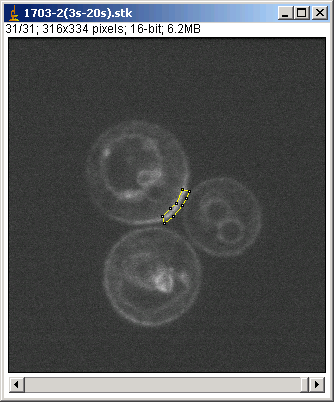
\includegraphics[width=0.3\textwidth]{fig/fig2321a_frapimage.png}}
 \subfloat[]{\label{fig:frapimage}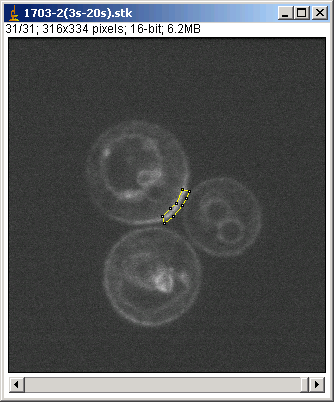
\includegraphics[height = 60mm]{fig/fig2321a_frapimage.png}}
 \quad
 \subfloat[]{\label{fig:frapmeasured}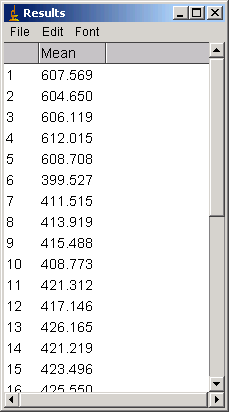
\includegraphics[height = 60mm]{fig/fig2321b_frapResults.png}}
 \caption{Measuring Stack Intensity Series. (a) Setting a Segmented ROI at the FRAPped area. (b) Results of Measuring Mean Intensity Dynamics.}
 \label{fig:frapresults}
\end{figure}


Measurement parameters can be added as argument by modifying the line 4 in the code 10. "Set Measurement" could be added with more parameters to be measured, and decimals could be increased (highlighted in bold).
\begin{indentCom}
\textbf{run}("Set Measurements\ldots", "  mean min integrated redirect=None decimal=4")
\end{indentCom}

\begin{indentexercise}{1}
Modify code 10 to include more measurement parameters (whatever you like), and test the macro. Check the results. 
\end{indentexercise}

% figure
\begin{figure}[htbp]
\begin{center}
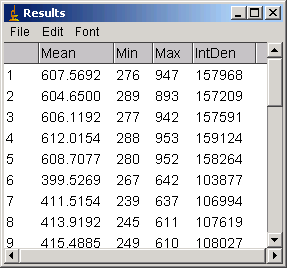
\includegraphics[scale=0.5]{fig/fig2322_moreResultsTable.png}
\caption{An example result after adding more measurement parameters.}
\label{fig_MoreMeasurementPara}
\end{center}
\end{figure} 

\subsection{Loop: while-looping}

Another way of letting part of macro to loop is \textbf{while}-statement. In this case, iteration is not defined strictly. Looping continues until certain condition is met. As soon as the condition is full-filled, macro interpreter goes out from the loop.

\subsubsection{Basics of while statement}
Here is a simple example macro using \ilcom{while}.
\lstinputlisting[morekeywords={*, while}]{code/code11.ijm}
This macro prints out characters 0 to 90 with a 10 increment. 

%figure
\begin{figure}[htbp]
\begin{center}
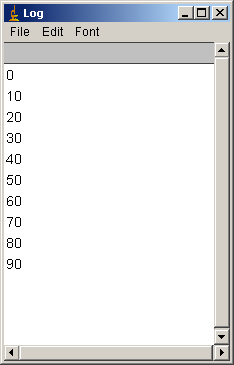
\includegraphics[scale=0.4]{fig/fig2331_Code11out.png}
\caption{Output of code 11}
\label{fig:code11 output}
\end{center}
\end{figure} 

\begin{itemize}
\item line 3: The macro interpreter first assigns 0 to the counter.
\item line 4: The interpreter evaluates if the counter value is less than or equal to 90. Since counter is initially 0\ldots 
\item line 5 Printing function is executed. 
\item line 6: counter is added with 10. 
\item line 7: the interpreter realizes the end of "while" boundary and goes back to line 4. Since counter= 10 <= 90, line 5 is again executed\ldots and so on. When counter becomes 100 in line 6 after several more loops, counter is no longer <=90. So the interpreter goes out from the loop, moves to line 8. Then the macro is terminated.
\end{itemize}

Line 5 could be written in the following way as well.
\begin{lstlisting}[numbers=none]
counter += 10;
\end{lstlisting}
This means that "counter" is added with 10. Similarly, subtracting 10 from counter is 
\begin{lstlisting}[numbers=none]
counter -= 10;
\end{lstlisting}
Multiplication is 
\begin{lstlisting}[numbers=none]
counter *= 10;
\end{lstlisting}
Division is
\begin{lstlisting}[numbers=none]
counter /= 10;
\end{lstlisting}
If the increment is 1 or -1, (counter +=1 or counter-=1), then one could also write them  as 
\begin{lstlisting}[numbers=none]
counter++;
 or 
counter--;
\end{lstlisting}
These two last macro functions are said to work faster than +=1 or -=1, but I myself do not see much difference. Computer is fast enough these days. 

\begin{indentexercise}{1}
(1) Try changing code 11 so that it uses "+=" sign.\\
(2) Change code 11 so that it uses "++" sign, and prints out integers from 0 to 9.\\
\end{indentexercise}
Evaluation of \ilcom{while} condition could also be at the end of loop. In this case, \ilcom{do} should be stated at the beginning of the loop. With do-while combination, the loop is always executed at least once, regardless of the condition defined by \ilcom{while} since macro interpreter reads lines from top to bottom. Try with the following exercise.

\begin{indentexercise}{2}
Change line 4 of code 11 to \ilcom{while (counter <0)} and check the effect (see below).
\end{indentexercise}

\lstinputlisting[morekeywords={*, while}]{code/code11_5.ijm}

Condition for the while-statement could be various. Here is a small list of comparison operators.

\begin{indentCom}
 \begin{tabular*}{0.5\textwidth}{ l r }
< & less than \\
<= & less than or equal\\ 
> & greater than\\ 
>= & greater than or equal to\\
== & equal\\
!= & not equal\\
 \end{tabular*}
\end{indentCom}

\begin{indentexercise}{3}
Modify code 11 so that the macro prints out numbers from 200 to 100, with an increment of -10. 
\end{indentexercise}

\subsubsection{Why is there while-loop?}

An often raised question with while-loop is why do we have two types of loops, 
the for-loop and the while-loop. Answering to this question, they have different
flexibility. For-loop is rather solid and while-loop is more flexible. In the
example code below, the user is asked for a correct number and if the answer is wrong, the
question is asked 5 times repeatedly. Number of loop is not determined by the
programmer, but interactively when the code is running. We will study
branching of the program based on if-else in the next section.  

\lstinputlisting[morekeywords={*, while}]{code/code11_6.ijm}

Writing a similar code using for-loop is possible but the code becomes tricky.
Below is the for-loop version of the above code.  

\lstinputlisting[morekeywords={*, for}]{code/code11_7.ijm}

Note that the third argument of for-loop is missing. Since variable
\ilcom{correct} does not change as long as the answer is wrong, we leave it not
incrementing nor decrementing. In such case we can leave the third argument
vacant. 

\subsection{Conditions: if-else statements}
\subsubsection{Introducing if-else}
A macro program could have parts which are executed depending some
conditions.
Here is an example of macro with conditions.
\lstinputlisting[morekeywords={*, if}]{code/code12.ijm}
\begin{itemize}
\item Line 3 The macro asks user to input a number and the number is substituted to the variable input\_num.
\item Line 4 Content of input\_num is evaluated. If input\_num is equal to 5, line 5 is executed and prints out the message in the Log window. Otherwise macro interpreter jumps to line 7, and ends the operation.  By adding "else" which will be executed if input\_num is not 5, the macro prints out message in all cases (see code 12.5 for this if - else case). 
\item Line 4 We used double equal signs for comparison (e.g. "if (a==5)"
). Note that this functional role is different from assignments, or substitution (e.g. "a = b + c").
\end{itemize}
%figure
\begin{figure}[htbp]
\begin{center}
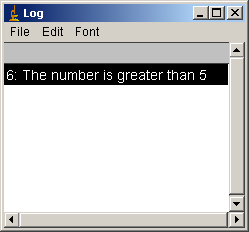
\includegraphics[scale=0.6]{fig/fig2341_code12out.png}
\caption{Output of code 12}
\label{fig:code12 output}
\end{center}
\end{figure} 

Now, we examine the content between 
parenthesis after ``if'' in more detail. 
Write the following code in your script editor and run it.
\lstinputlisting[morekeywords={*, ==}]{code/code12_1.ijm}
The output in the log window should be \textit{1} indicating that ``\ilcom{(5 ==
5)}'' is \textit{1}. Next, modify the code like below and run it.
\lstinputlisting[morekeywords={*, ==}]{code/code12_2.ijm}
The output is now 0, indicating that ``\ilcom{(5 == 4)}'' is
0.
What double equal signs \ilcom{==} are doing in these
examples are comparison of numbers in the left and the right side, and if
the number is same, it returns 1 and if they are not equal, it returns 0. 1 and
0 actually are representing \textbf{true} (= 1) or \textbf{false} (= 0), the
\textbf{boolean values}.

We could also test if they are NOT equal. For this, replace \ilcom{==} by
\ilcom{!=}.
\lstinputlisting[morekeywords={*, !=}]{code/code12_3.ijm}
Run the code above, and it returns 1, because 5 is NOT 4 and that is true. Now,
you could introduce the \textit{if} again as follows.
\lstinputlisting[morekeywords={*, if, else}]{code/code12_35.ijm}
In the parenthesis after ``if'', there is obvious TRUE statement (5 is not 4).
This is true, so the macro function bounded by curly braces is executed, which is to
print out ``true!'' in the log window.

Try changing the line two to \ilcom{if (5 == 4)}. Running this prints nothing
in the log window, because 5 is not 4 (FALSE!) so that the macro function in
the line 3 is ignored. To avoid such ignorant no-output behavior, you could add
``else'' as follows.

\lstinputlisting[morekeywords={*, if, else}]{code/code12_4.ijm}

The code works also with the direct true or false
declaration inside the if parenthesis. Try the follwoing code.

\lstinputlisting[morekeywords={*, if, else}]{code/code12_5.ijm}

The above prints two lines of ``false!'' in the log window. You could replace
the if parenthesis values to 1 and ture to check that it works as well. 

By now, you probably are pretty clear with what is going on in the code below. 
\lstinputlisting[morekeywords={*, if, else}]{code/code12_6.ijm}

\subsubsection{Complex Conditions}
In many cases, you might need to evaluate the condition of multiple variables at once. 
For such demands, several different comparisons can be combined by using following Boolean operators. 

\begin{indentCom}
 \begin{tabular*}{0.5\textwidth}{ l l }
\&\& & boolean AND\\
|| & boolean OR\\
\end{tabular*}
\end{indentCom}

Let's first test what they do with very a simple example directly using
\ilcom{true} and \ilcom{false}.
\lstinputlisting[morekeywords={*, if, else}]{code/code12_65.ijm}
When you run this code as it is, line 4 and line 8 are both executed and prints
the messages. For the first \ilcom{if} parenthesis, \ilcom{\&\&} operator tests if
both sides are true. If both are indeed true, it returns true (1), and that is
the case above. If one of them or both are false, then \ilcom{\&\&}
operator returns false(0). 

On the other hand, in the second if parenthesis,
\ilcom{||} operator tests if one of the two sides is true. Since both are
true in the above code, OR operator returns true because at least one of them is
true. Only when both sides are false, the returned value becomes false (0).

\begin{indentexercise}{1}
Change the values of \ilcom{a} and \ilcom{b} in code 12\_65 to \ilcom{false} and
compose other three possible combinations (e.g. a = true, b = false will print
only one line).
Check the output. Change the values of \ilcom{a} and \ilcom{b} also to 0 and/or
1 and check the results. 
\end{indentexercise}

Here is a bit more realistic example (though very useless), an extended version
of code 16\_6.
\lstinputlisting[morekeywords={*, if, else}]{code/code12_75.ijm}
\begin{itemize}
\item Line 4 and 5 Ask user to input two parameters.
\item Line 6 is for setting a string variable, to abbreviate a long string assignment that appears four times in the macro.
\item Line 7 evaluates these input parameters by comparing each of them separately, but the decision is made by associating two decisions by "\&\&". 
\item Text after "//" is called comment. Text after this double slash will not be evaluated by the macro interpreter. Comments helps programmers later for remembering (or letting other programmer to understand) the purpose of the line. 
\item Line 10, != compares left and right sides of the operators and returns true if they are NOT equal.   
\end{itemize}
From line 10 to 17, there are several layers of conditions. Macro programmer should use tab-shifting for deeper condition layers as above for the visibility of code. Easy-to-understand code helps the programmer oneself to debug afterward, and also for other programmers who might reuse the code.
\subsubsection{Application of if-statement}
\label{sec:dotmove}

We write a macro that produces an animation of moving dot. User inputs the speed
of the dot, and then the animation is generated. In the animation (which
actually is a stack) the dot moves horizontally and bounces back from the edge
of the frame. \ilcom(if) operator is used to switch the movement direction.
\lstinputlisting[morekeywords={*, setForegroundColor, setBackgroundColor, if}]{code/code13.ijm}

\begin{itemize}
\item Lines 4 to 11: Set parameters for drawing a dot. It is also possible to directly use numerical values in the later lines, but for the sake of readability of the code, and also for possible later extension of the code, it is always better to use easy-to-understand variables and explicitly define them like in these lines. 
\end{itemize}
A short note on the x-y coordinate system in digital images: Since digital image is a matrix of numbers, each pixel position is represented as coordinates. The top left corner of image is the position (x, y) = (0, 0). X increases horizontally towards right side of the image. Y increases vertically towards the bottom of the image.  In line 9, y-position of the dot is defined to be placed in the middle of the vertical axis. 
\begin{itemize}
\item Lines 14, 15: These lines set the drawing and background color. Three arguments are for each RGB components. Here the image is in grayscale so all the RGB components are set to the same value. 0 is black, and int = 255 = white.
\item Line 14 asks the user to input the speed of the dot movement.
\item Lines 16, 17 prepares a new stack with parameters defined in lines 7, 8 and 9.
\item Lines 21 to 34 is the loop for drawing moving dot. Loop will be iterated from the starting frame until the last frame. Line 21 creates an oval ROI, which will be filled in line 22 with the foreground color that was already set in the line 14. \ilcom{makeOval} function is explained in the Built-on function page as follows.

\begin{indentCom}
\textbf{makeOval}(x, y, width, height)\\
Creates an elliptical selection, where (x,y) define the upper left corner of the bounding rectangle of the ellipse. 
\end{indentCom}
\item Line 27: Shifts the x position of the dot by ``speed'' distance. 
\item Line 28: if the position calculated in the line 27 exceeds the boundary, either left \ilcom{(x\_position < 0)} OR right \ilcom{(x\_position > (w-sizenum))}, then the direction of movement is switched by multiplying -1.
\end{itemize}
\begin{indentexercise}{2}
Modify code 13 that the dot moves up and down vertically. Change the stack width and height as well. 
\end{indentexercise}

\subsection{String Arrays}
Array is a powerful tool. before going into how to use it, here is an easy explanation. 
Imagine that an array is a stack of boxes. Boxes could contain either numbers or strings. 
For instance, if you have a following list of strings:

\textit{Heidelberg, Hamburg, Hixton, Grenoble, Monterotondo}

An array "EMBL" could be prepared that the array element will contain these 5 strings. 

 %figure
\begin{figure}[htbp]
\begin{center}
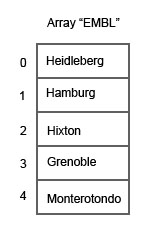
\includegraphics[scale=0.6]{fig/fig2441_arrayScheme.jpg}
\caption{EMBL array}
\label{figEMBLarray}
\end{center}
\end{figure} 
 
Then when you want to retrieve some name, you refer to the address within the array. 
So EMBL[0] will be Heidelberg, EMBL[4] will be Monterotondo, and so on. 
In such a way, files names contained in a folder could be listed and stored, 
or x-y coordinates of free-hand ROI could be stored for further use. 

Here is a macro using the EMBL array example. 

\lstinputlisting[morekeywords={*, newArray}]{code/code20.ijm}

\begin{itemize}
\item Line 3 uses a function that creates a new array (\ilcom{newArray()}),
defined by a parameter for number of array elements (in the example case its 5) and its name \ilcom{EMBL}.
\item From line 4 to 8, each array from position 0 to 4 will be filled with
names (Array starts with 0th element).
\item Line 9 asks the user to input the address (position) within the array.
Then this input address is examined if the address exists within the
\ilcom{EMBL} array in line 10. \ilcom{EMBL.length} returns the number of "boxes"
within the array. If this is satisfied, then line 10 prints out the string in that address.
\end{itemize}

Array could be created and initialized with actual values at the
same time, so line 3 to 8 could be written in a single line like this: 
\begin{lstlisting}[numbers=none]
EMBL = newArray("Heidelberg","Hamburg","Hixton","Grenoble","Monterotondo");
for (i = 0; i < EMBL.length; i++)
    print(EMBL[i]);
\end{lstlisting}

\subsection{Numerical Array}

Array could also contain numerical values, and this way of usage is more common when you do image analysis. Here is a simple example of numerical array that prints out intensity profile along selected line ROI. 

\lstinputlisting[morekeywords={*, newArray, selectionType, getProfile, setResult, updateResults}]{code/code20_5.ijm}

\begin{itemize}
\item Line 3: Check if the selection type is a straight line ROI. If not, macro terminates leaving a message. 

\begin{indentCom}
\textbf{selectionType}()\\ 
Returns the selection type, where 0=rectangle, 1=oval, 2=polygon, 3=freehand, 4=traced, 5=straight line, 6=segmented line, 7=freehand line, 8=angle, 9=composite and 10=point. Returns -1 if there is no selection.
\end{indentCom}

\item Line 4: Empty array \ilcom{tempProfile} is loaded with the intensity profile along the line ROI by \ilcom{getProfile}().
\item
\begin{indentCom}
\textbf{getProfile}()\\
Runs Analyze/Plot Profile (without displaying the plot) and returns the intensity values as an array.
\end{indentCom}

\item Line 5: Passing the array \ilcom{tempProfile} to function "output\_results", which prints the content of array in Results window. 

\item Line 7 to 14: A function for outputting the profile array in the result table. It takes an argument \ilcom{rA}, which is supposed to be an array. 
\item Line 8: Clears the result table. 
\item Line 9 to 12: for-loop to go through the array and to print out each element. 
\item Line 10: Sets the pixel position along the segment in the column labeled "n". 
\item Line 11: Sets the content of the array (pixel intensity) in the column labeled "intensity".

\begin{indentCom}
\textbf{setResult}("Column", row, value)
Adds an entry to the ImageJ results table or modifies an existing entry. The first argument specifies a column in the table. If the specified column does not exist, it is added. The second argument specifies the row, where 0<=row<=nResults. (nResults is a predefined variable.) A row is added to the table if row=nResults. The third argument is the value to be added or modified. 
\end{indentCom}
\item Line 13: Updates the result table, so that above changes are actually reflected in the Result window. 

\begin{indentCom}
\textbf{updateResults}()
Call this function to update the "Results" window after the results table has been modified by calls to the setResult() function. 
\end{indentCom}
\end{itemize}

\begin{indentexercise}{1}
Modify code 20.5 that the macro calculates the sum of all intensity.\\
\begin{enumerate}
\item You do not need the function anymore. 
\item for-loop should be used.
\item Hint: use \ilcom{tempProfile.length}
\end{enumerate}
\end{indentexercise}

\subsection{Array Functions}

Arrays could be directly treated using arary funcitons. These functions are:
\begin{shaded}\begin{indentCom}
\item \textbf{Array.concat(array1,array2)} Returns a new array created by
joining two or more arrays or values. 
\item \textbf{Array.copy(array)} Returns a copy of array. 
\item \textbf{Array.fill(array, value)} Assigns the specified numeric value to
each element of array.
\item \textbf{Array.getStatistics(array, min, max, mean, stdDev)} Returns the
min, max, mean, and stdDev of array, which must contain all numbers.
\item \textbf{Array.print(array)} Prints the array on a single line. 
\item \textbf{Array.rankPositions(array)} Returns, as an array, the rank
positions of array, which must contain all numbers or all strings. 
\item \textbf{Array.reverse(array)} Reverses (inverts) the order of the
elements in array. 
\item \textbf{Array.slice(array,start,end)} Extracts a part of an array and
returns it. 
\item \textbf{Array.sort(array)} Sorts array, which must contain all numbers
or all strings. String sorts are case-insensitive in v1.44i or later.
\item \textbf{Array.trim(array, n)} Returns an array that contains the first n
elements of array.
\end{indentCom}\end{shaded}
For example, array could be sorted and reversed.
\begin{lstlisting}[numbers=none]
EMBL = newArray("Heidelberg","Hamburg","Hixton","Grenoble","Monterotondo");
Array.print(EMBL);
Array.sort(EMBL);
Array.print(EMBL);
Array.reverse(EMBL);
Array.print(EMBL);
\end{lstlisting} 
The output of this code is:
\begin{lstlisting}[numbers=left]
Heidelberg,Hamburg,Hixton,Grenoble,Monterotondo
Grenoble,Hamburg,Heidelberg,Hixton,Monterotondo
Monterotondo,Hixton,Heidelberg,Hamburg,Grenoble
\end{lstlisting} 
The first line is printed in the order when the array was initialized. After
sorting, names are in alphabetical order. Third line shows the reversed
elements. 

\subsection{Application of Array in Image Analysis}

Array is used in many built-in macro functions, especially for storing array of numerical values. Here is a list of functions which use array. 

\begin{indentCom}
\texttt{
\item Dialog.addChoice("Label", items) 
\item Dialog.addChoice("Label", items, default)
\item Fit.doFit(equation, xpoints, ypoints)
\item Fit.doFit(equation, xpoints, ypoints, initialGuesses)
\item getFileList(directory)
\item getHistogram(values, counts, nBins[, histMin, histMax])
\item getList("window.titles")
\item getList("java.properties")
\item getLut(reds, greens, blues)
\item getProfile()
\item getRawStatistics(nPixels, mean, min, max, std, histogram)
\item getSelectionCoordinates(xCoordinates, yCoordinates)
\item getStatistics(area, mean, min, max, std, histogram)
\item makeSelection(type, xcoord, ycoord)
\item newArray(size)
\item newMenu(macroName, stringArray)
\item Plot.create("Title", "X-axis Label", "Y-axis Label", xValues, yValues)
\item Plot.add("circles", xValues, yValues)
\item Plot.getValues(xpoints, ypoints)
\item setLut(reds, greens, blues)
\item split(string, delimiters) 
}
\end{indentCom}

To learn the actual use of Array in Image analysis, we use some of these functions and 
create a macro that reads and shows the line-profile from segmented line ROI. 
In recent version of ImageJ, selection thickness controls the width of segmented
line ROI when you do \ijmenu{[Analyze > Plot Profile])}. We try to mimick this
behavior in macro, and instead of choosing the line ROI thickness using GUI, the
macro asks the user to input the thickness. 

In the code below, there is only one macro. Two functions are added at the
bottom. One is for profile plotting and the last one is for listing
intensity profile data in the result table. Strategy of this macro is to use
straight line selection for each segment, measure that segment and then profiles
are concatenated to the total profile array.

%\lstinputlisting[morekeywords={*, newArray, selectionType, getProfile, setResult, updateResults}]{code/code20_75.ijm}
%\lstinputlisting[morekeywords={*, getSelectionCoordinates, makeLine, Plot,
% create, setLimits, setColor, add, show}]{code/code20_75.ijm}
\lstinputlisting[morekeywords={*, getSelectionCoordinates, makeLine, Plot,
create, setLimits, setColor, add, show, Array, concat,
getStatistics}]{code/code20_76.ijm}

\begin{itemize}
\item Lines 2 - 16: Main part, macro for the segmented line ROI measurement.  

\item Line 3: Check if the selection type is a segmented line ROI. If not, macro
terminates leaving a message.

\item Line 4: Reads the x and y coordinates of the segmented line
and store them in two arrays \ilcom{xCA} and \ilcom{yCA}.

\begin{indentCom}
\textbf{getSelectionCoordinates(xCoordinates, yCoordinates)}\\
Returns two arrays containing the X and Y coordinates of the points that define the current selection. 
\end{indentCom}

\item Line 5 - 7: Asks the user to input width of the segmented ROI. The ROI
line width is set to that value.

\item Line 8: A new array \ilcom{totalprofile} is created, initialized without
any element. This new array will store the profile data of full ROI.

\item Line 9 - 13: Profile measurement by placing straight line ROI,
for wach segment of the original ROI. \ilcom{makeLine} function is used for this
purpose, and \ilcom{getProfile} returns intensity profile of the corresponding
line ROI. Profile data in \ilcom{thisprofile} array are concatenated to
\ilcom{totalprofile} array using \ilcom{Array.concat}.

\begin{indentCom}
\textbf{makeLine(x1, y1, x2, y2)}\\
Creates a new straight line selection. The origin (0,0) is assumed to be the upper left corner of the image. Coordinates are in pixels. With ImageJ 1.35b and letter, you can create segmented line selections by specifying more than two coordinate, for example makeLine(25,34,44,19,69,30,71,56).
\end{indentCom}

\item Line 14: Call graph plotting function (Line 20 - 27), passing
\ilcom{totalprofile} array as an argument.

\item Line 15: call function to printout the profile array in the results window
(Lines 32 - 39).

\item Line 20 - 27: Function for plotting the intensity profile.
\item Line 21 : Use \ilcom{Array.getStatistics} function to know the minimum and
the maximum value of the array that was given as argument.
\item Line 22: Creates the window and axes of the plot. 
\item Line 23: Set the range for x and y axis using the results of line 21
\ilcom{min} and \ilcom{max}. 5\% of offset is added to both values for some
margins below and above.
\item Line 24: Sets the color of the plot. 
\item Line 25: Plot the profile. 
\item Line 26: Show the plot on the screen (lot is hidden until this show()
function).

\item Line 30 - 37: Function for outputting the profile array in the result
table. This function is exactly the same function you already used in the
previous chapter (code 20.5).

\end{itemize}


\subsection{Working with Strings}

With some advanced macro programming, you might need to manipulate Strings (texts) from your code. For example, let's think about a title of an image ``exp13\_C0\_Z10\_T3.tif''. Such naming occurs often to indicate that this image is from third time point, at 11th slice (imagine that the Z slice numbering starts from 0) and its first channel. 

We might be lucky enough to read out dimensional information from header, but quite often such information is only available in the file name (the title of the image). To extract dimensional information from file name, we need to know how to deal with strings in macro to decompose those strings and extract information that we need. Build-in macro functions which are related to such tasks with strings are the following. 

\begin{itemize}
\item lengthOf(str)
\item substring(string, index1, index2)
\item indexOf(string, substring)
\item indexOf(string, substring, fromIndex)
\item lastIndexOf(string, substring)
\item startsWith(string, prefix)
\item endsWith(string, suffix)
\item matches(string, regex)
\item replace(string, old, new)
\end{itemize}

Let's go back to the example file name ``exp13\_C0\_Z10\_T3.tif'' again. If we need to get the file name without file extension, what should we do? Several ways are there, but lets start with the simplest one. We assume that we already know that all the file names we are dealing with are TIFF format, so we know that they all ends with ``.tif''. So we could replace the ``.tif'' with a 0 length string. we could do this by using \ilcom{replace}. 

\begin{lstlisting}
name = "exp13_C0_Z10_T3.tif";
newname = replace(name, ".tif", "");
print(newname);
\end{lstlisting}

This will print out "exp13\_C0\_Z10\_T3" in the log window. In the second line, the function \ilcom{replace} is used. The old string ".tif" is replaced by a new 0 length string "". So it works! 

But what if our lucky assumption that all files ends with ".tif" is not true and it could be anything? To work with this, we now need to use different strategy to now the file extension. By definition, file extension and the file name is separated by a dot. Length of the extension could be various, as some extension such as python file is ".py" and C code is ".c". Thus, we cannot assume that the length of the file extension is constant, but we know that there is a dot. 

For such case with variable length of file extension being expected, we first need to know about the \textbf{index} of the dot within file name. Each character within file name is positioned at certain index from the beginning of the name. In the example we are now dealing with, The index 0 is ``e''. The index 1 is ``x''. The index starts from 0. Since the index starts from 0, the last index will be total length of the file name minus one. You could modify the code above like below to try getting the length of the file name. 

\begin{lstlisting}
name = "exp13_C0_Z10_T3.tif";
tlength = lengthOf(name);
print(tlength);
\end{lstlisting}

You should see ``19'' in the log window. That is the length of this file name. So in this example string, index starts from 0 and the last index is 18. 

Next, you need to know is about the function \ilcom{substring(string, index1, index2)}. With this function, you could extract part of the \ilcom{string} by the start index and the end index. We could just try this by again modifying the code above. 

\begin{lstlisting}
name = "exp13_C0_Z10_T3.tif";
subname = substring(name, 0, 3);
print(subname);
\end{lstlisting}

In the log window, there should be ``exp''. The second argument in the code above is 0, and the third is 3. This tells the substring function to extract characters from the index 0 to index 2 should be extracted (so the third argument will be the index just after the last index that would be included in the substring). 

\begin{indentexercise}{1}
Test changing the second and the third argument so that different part of the file name is extracted. 
\end{indentexercise}

So how do we know the index of dot? For this we use the \ilcom{indexOf(string, substring)}. Try the following code. 

\begin{lstlisting}
name = "exp13_C0_Z10_T3.tif";
dotindex = indexOf(name, ".");
print(dotindex);
\end{lstlisting}

Now you know that the index of dot is ``15''. We could then combine the knowledge we have now to compose a single macro that extracts the filename without file extension. 

\begin{lstlisting}
name = "exp13_C0_Z10_T3.tif";
dotindex = indexOf(name, ".");
filename = substring(name, 0, dotindex);
print(filename);
\end{lstlisting}

Let's make the problem a bit more complicated. If the file name contains multiple dots, what should we do? In the example below, I added two more dots. 

\begin{lstlisting}
name = "exp13._C0._Z10_T3.tif";
dotindex = indexOf(name, ".");
filename = substring(name, 0, dotindex);
print(filename);
\end{lstlisting}

Output is now ``exp13''. Far from what we need. To treat such case, we use \ilcom{lastIndexOf}, which returns the index of the last appearance of the given character. Let's slightly modify the code. 

\begin{lstlisting}
name = "exp13._C0._Z10_T3.tif";
dotindex = lastIndexOf(name, ".");
filename = substring(name, 0, dotindex);
print(filename);
\end{lstlisting}

It should then working again as we want. 

Let's change our task: We now want to know the time point that this image was taken. How should we do that? Examining the file name again, we realize that the time point number appears after ``T''. The number could be any length of digits, but currently is 0. Then the dot comes right after the number. We then just need to know the index of ``T'' \ldots but wait, we might have ``T'' anywhere, as this is a single character alphabet that could easily be a file name. Therefore we find the index of ``\_T'' that looks like more specific. 

\begin{lstlisting}
name = "exp13._C0._Z10_T3.tif";
timeindex = indexOf(name, "_T");
print(timeindex);
\end{lstlisting}

Now we know that ``\_T'' is at index 14, so the number should start from the index 16 (because index 15 will be ``T''). Taken this into account, we could extract the time point. 

\begin{lstlisting}
name = "exp13._C0._Z10_T3.tif";
timeindex = indexOf(name, "_T");
dotindex = lastIndexOf(name, ".");
timepoint = substring(name, timeindex + 2, dotindex);
print(timepoint);
\end{lstlisting}

The time point that you have just now captured is a string. You can not pass this to mathematical assignments. To do so, you need to convert this to a number. For doing so, you could use \ilcom(parseInt(string)). 

\begin{lstlisting}
name = "exp13._C0._Z10_T3.tif";
timeindex = indexOf(name, "_T");
dotindex = lastIndexOf(name, ".");
timepoint = substring(name, timeindex + 2, dotindex);
timepoint = parseInt(timepoint);
print(timepoint * 2);
\end{lstlisting}

An example case where conversion of string to number (in this case an integer) required is when you need to compare such file names and get the maximum time point from all the file names. Usage is diverse, but at some point you need to use this. If you need a Float number (numbers with decimal point), use \ilcom{parseFloat(string)}



\clearpage

\section{Measurement of Nucleus Periphery Intensity}

We now shift to a more actual task for learning the ImageJ macro programming. 

\subsection{What we will do here}

We take an example 2Channel images with histone signal and nuclear pore complex (NPC) protein signal. There are two images from different time points. 
\begin{itemize}
\item NPC\_T01.tif
\item NPC\_T15.tif
\end{itemize}

\begin{figure}[h!]
 \centering
 \subfloat[Time point 1]{\label{fig:NucTimePoint1}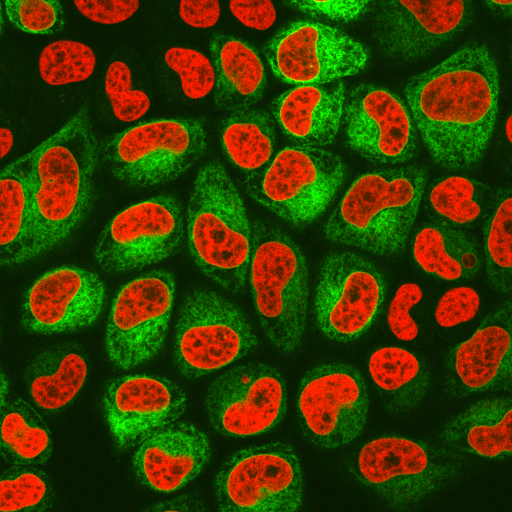
\includegraphics[width = 0.45\textwidth]{fig/NPC_T01.png}} 
 \quad
 \subfloat[Time point 15]{\label{fig:NucTimePoint15}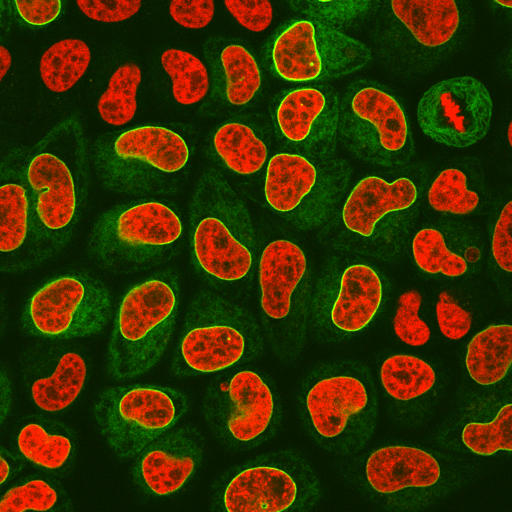
\includegraphics[width = 0.45\textwidth]{fig/NPC_T15.png}} \\
 \caption{NPC localization difference at two time points: Histone (Red) and NPC (Green) channels are shown. Compard to the first time point, NPC is more concentrated in nucleus periphery at time point 15. }
 \label{fig:NucMeasure}
\end{figure}

Our task is to compare NPC signal intensity in the nuclear periphery at these two time points. The original data is a time lapse sequence showing a process of NPC protein relocalizing from cytoplasm to the nuclear membrane. Above two images are from the first and the last time points\footnote{The original 4D hyperstack file is NPCsingleNucleus.tif. You could load the file via CourseModule plugin.}. 

Following is the outline of our protocol. 
\begin{enumerate}
    \item Split channels, blur nucleus a bit then segment nucleus by thresholding.
    \item Use particle analysis to get nucleus ROIs
    \item (looping) Increase the ROI line width and then convert ROIs from areas to lines.
    \item Combine all ROIs and create a single ROI. 
    \item Measurement of NPC signal intensity using the ROI.
    \item Print out mean intensity of NPC signal in nuclear periphery for that frame.  
\end{enumerate}

In this protocol, we use ROI manager extensively.  

\begin{figure}[h!]
 \centering
 \subfloat[Original NPC Image, Channel1]{\label{fig:originalNPC}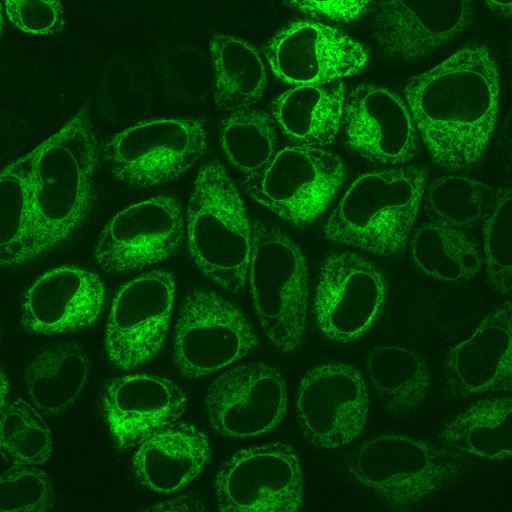
\includegraphics[width = 0.45\textwidth]{fig/NPC_T1npc.png}} 
 \quad
 \subfloat[Original Nucleus Image, Channel 2]{\label{fig:originalNuc}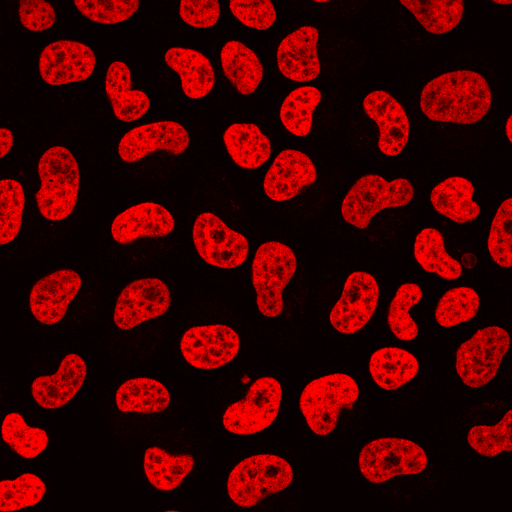
\includegraphics[width = 0.45\textwidth]{fig/NPC_T1nuc.png}}
\\
 \subfloat[Thresholded Image]{\label{fig:binarizedNuc}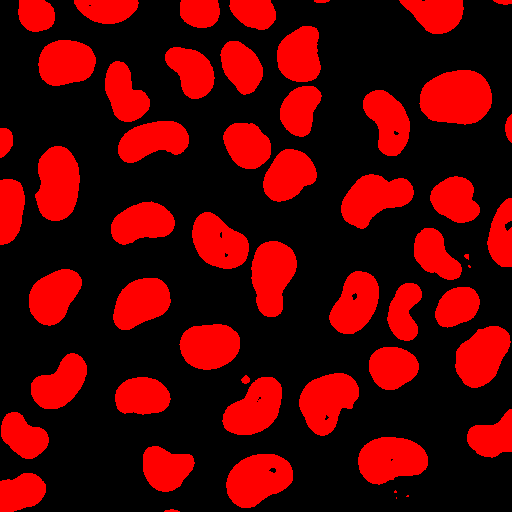
\includegraphics[width = 0.45\textwidth]{fig/NPC_T1thresholded.png}}
 \quad
 \subfloat[NPC with band ROIs]{\label{fig:NPCbandRois}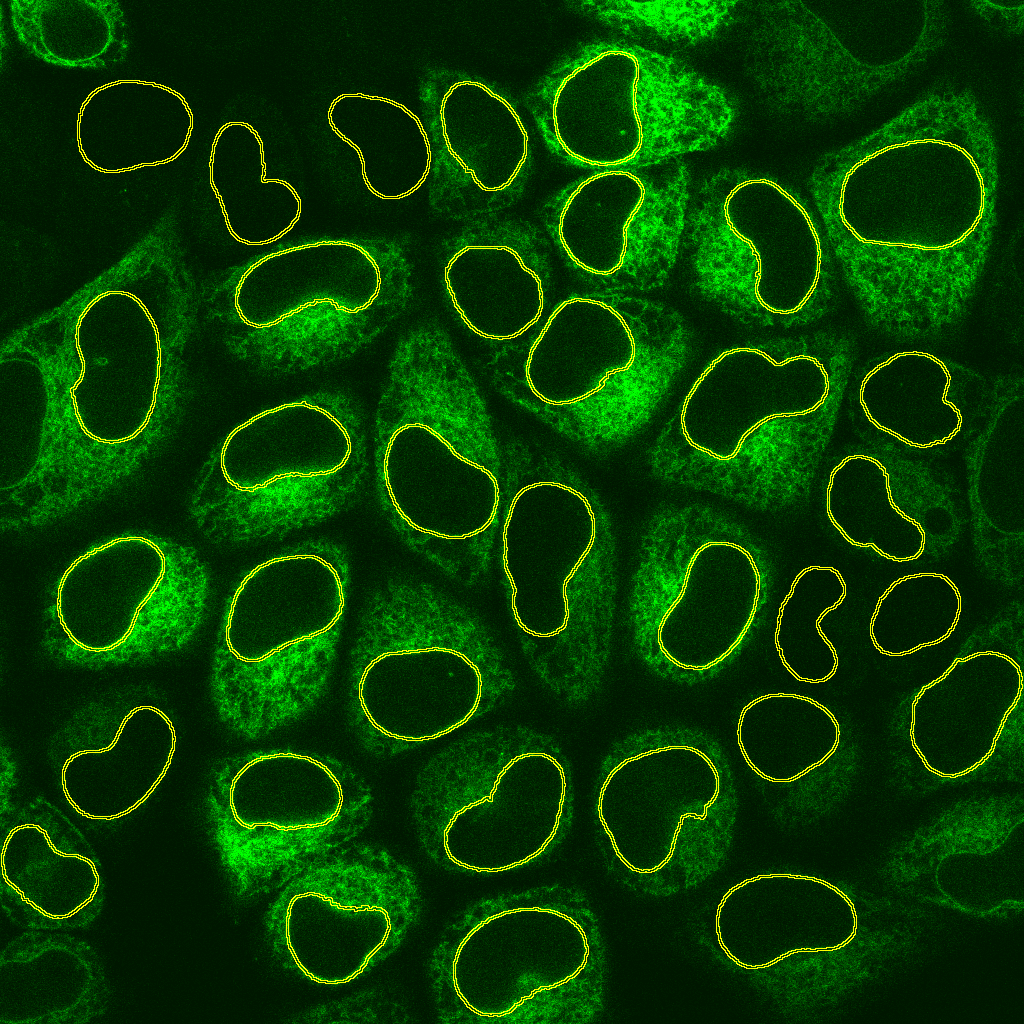
\includegraphics[width = 0.45\textwidth]{fig/NPC_resultsChNPC.png}}
 \caption{Steps of measurement.}
 \label{fig:nucsegProc}
\end{figure}

\subsection{Step-by-Step Actual Macro Writing}

Here is the step-by-step protocol. Load the image stack \textbf{NPC\_01.tif} and follow the instructions. Don't start writing a macro immediately, try the first half of the procedure (down until ``Analyze Particles'') manually without command recorder. After you are convinced that it works, start \ijmenu{[Plugins > Macros > Record]} to record the commands.  When you record functions, be sure that Macro is selected in ``Record:'' drop down menu at the top-left corner of the recorder.

It is always good to write several lines and then test run the part immediately. In this way you could easily fix the code if there is error. Macro basically is executed line by line, so you could incrementally write a line and test it. 

The latter half is difficult to do / cannot do from the ImageJ menu. For this part, you should write the code without recording. 

It is rather long but mostly due to the detailed explanation of what is going on for each step. You could check the final code first (appears in the final part of this section) so that the actual coding you need to do is not so long. In addition, if you once write a macro everything could be done by running the macro in a matter of a single click of ``Run'' button in the script editor. 

\begin{enumerate}
  \item Split channels (fig. \ref{fig:nucsegProc} a, b): \\ \ijmenu{[Image > Color > Split Channels]}
  \begin{itemize}
	\item In the Recorder, you would see the following macro functions in the history. 
\begin{lstlisting}[numbers=none]
run("Split Channels");
\end{lstlisting}
	\item ``run'' function is the most frequently used build-in macro function. 

\fbox{
\parbox[b][18em][c]{0.80\textwidth}{
  \textbf{run("command"[, "options"])}
  Executes an ImageJ menu command. The optional second argument contains values that are automatically entered into dialog boxes (must be GenericDialog or OpenDialog). Use the Command Recorder (Plugins>Macros>Record) to generate run() function calls. Use string concatentation to pass a variable as an argument. With ImageJ 1.43 and later, variables can be passed without using string concatenation by adding "\&" to the variable name.
}}

The run function takes menu item as the first argument, and optional values (values you fill in in dialog for many of the functions) in the second argument. In case of channel splitting, there is not option so the second argument is ignored. 
  \end{itemize}
  \item We now work on the nucleus image. Activate (Click a window to bring up to the top) Channel 2 (red, nucleus image).
  \begin{itemize}
	\item In the recorder, the function \ilcom{selectWindow("C1-NPC\_T1.tif");} appears. 
	\item Though this function works with this specific file, it does not work with different images. To generalize the macro we should combine this part with the channel splitting such that:
\begin{lstlisting}
orgtitle = getTitle();
run("Split Channels");
c1name = "C1-" + orgtitle;
c2name = "C2-" + orgtitle;
selectWindow(c2name);
\end{lstlisting}
	\item  \textbf{Details:} To activate an image in macro, the window should be specified in some way to activate that image. For this we use the build-in macro function \ilcom{setWindow(image title)}.  

\fbox{
\parbox[b][3em][c]{0.80\textwidth}{
  \textbf{selectWindow("name")}\\
Activates the window with the title "name".
}
}

This function takes a title of a window as an argument and activates that window. Since ``Split Channel'' has a standard behavior that it appends ``C1-'' or ``C2-'' or ``C3'' in front of the original image title, we can construct the name of the resulting images after channel splitting. How do we get the original image title? For this, there is a command \ilcom{getTitle()} which returns the image title as a string. 

\fbox{
\parbox[b][3em][c]{0.80\textwidth}{
\textbf{getTitle()}\\
Returns the title of the current image.
}
}

Putting these macro functions together, we can have the lines of  macro that splits a multi channel image and then select the nucleus channel as already shown above. 


\textbf{Optional: Do this if you have time.} \ilcom{setWindow} function is constrained by the image title. We could alternatively specify an image by ID number, not by its name. This is in many cases better since window title could be overlapped where as imageID is based on the window ID, so using image ID number avoids name clash. Each window has a unique ID number. A function \ilcom{getImageID()} captures the imageID of the currently active (top) window and returns that value. 

\fbox{
\parbox[b][8em][c]{0.80\textwidth}{
\textbf{getImageID()}\\
Returns the unique ID (a negative number) of the active image. Use the selectImage(id), isOpen(id) and isActive(id) functions to activate an image or to determine if it is open or active.
}
}

\begin{indentexercise}{1}
\textbf{getImageID() exercise:}
Open a new tab and test the code below and run it on different windows. Confirm that each window has different ID number. 
%\begin{lstlisting}[numbers=none]
\begin{lstlisting}
id = getImageID();
print( id );
name = getTitle();
print( name );
\end{lstlisting}
\end{indentexercise}

  \end{itemize}

  \item Blur the image to reduces noise.\\
 \ijmenu{[Process > Filter > Gaussian Blur]} and set sigma = 1.
  \begin{itemize}
	\item The macro function is 
\begin{lstlisting}[numbers=none]
run("Gaussian Blur...", "sigma=1");
\end{lstlisting}
	\item Here is another case of \ilcom{run} function, but this time with the second argument. Since Gaussian Blur command first calls a dialog pop-up which asks you for the size of the Gaussian kernel (sigma), the second argument in this function specifies the sigma value. You could test this one line code in a separate tab to test effect of changing the number of sigma. 
  \end{itemize}
  \item Binarize the image by Auto Local Threshold (fig. \ref{fig:binarizedNuc}).\\
 \ijmenu{[Image > Adjust > Auto Local Threshold...]}, Method "Mean", Radius = 100 and others are default value. 
  \begin{itemize}
	\item  The macro function is\\
\begin{lstlisting}[numbers=none]
run("Auto Local Threshold", "method=Mean radius=100 parameter_1=0 parameter_2=0 white");
\end{lstlisting}
  \end{itemize}
  \item Analyze Particles: \\
\ijmenu{[Analyze > Analyze Particles]}. Area: 100 - Infinity, Show nothing, check exclude edge particles,  include holes and add to RoiManager. 

\begin{figure}[h!]
\begin{center}
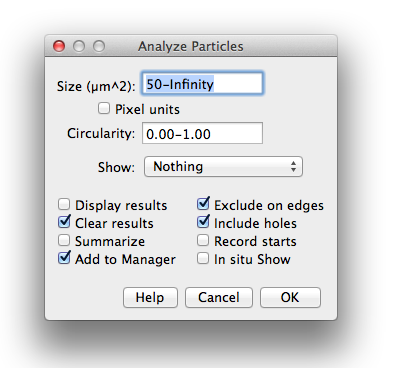
\includegraphics[width=0.6\textwidth]{fig/NPC_PAdialog.png}
\caption{Particle Analysis dialog}
\label{fig:padialog}
\end{center}
\end{figure}

  \begin{itemize}
	\item This operation extracts nucleus ROIs and store in ROI manager. At the same time this operation ignores garbages and other nucleus from being listed in ROI manager.
	\item The macro function is:\\
\begin{lstlisting}[numbers=none]  
run("Analyze Particles...", 
	"size=50-Infinity circularity=0.00-1.00 show=Nothing exclude clear include add");
\end{lstlisting}
	\item Here is the \ilcom{run} function again now with many more options in the second argument. With the ``Analyze Particle\ldots'' command, its dialog asks many options. All those options are now included in the second argument. We generally do not write all these things from scratch. We RECORD the function by giving command. Recording avoids mistakes and work loads, so use it as much as possible! \\
To use variables inside the argument, the best practice is to construct the option argument outside the run command. For example, above command could be rewritten as:
\begin{lstlisting}[numbers=none]
minsize = 50;
opt = "size=" + minsize + "-Infinity circularity=0.00-1.00 show=Nothing exclude clear include add";  
run("Analyze Particles...",  opt);
\end{lstlisting}
This renovation does not change the behavior of the previous single line version, but this change increases the readability. In addition, a new variable \ilcom{minsize} is explicitly defined so that it will be easy to change the allowed minimum size of the particle filtering. 
  \end{itemize}
  \item  We now have ROIs, but we need to convert them so that the ROI selects only the rim of nuclei, the peripheral zone of nucleus. To do this we need to work on each ROI one by one as conversion of ROI works only with single ROI\ldots you need to loop from here. 

\begin{figure}[h!]
\begin{center}
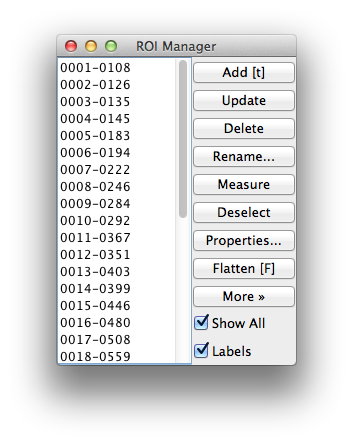
\includegraphics[width=0.6\textwidth]{fig/NPC_roManagerFilled.png}
\caption{Roi Manager with of Nucleus ROIs}
\label{fig:roimanagerFilled}
\end{center}
\end{figure}

  \item (in the loop) Select a ROI in the roi manager. 
  \begin{itemize}
  \item  the macro function is
\begin{lstlisting}[numbers=none]  
	roiManager("Select", i);
\end{lstlisting}

\fbox{
\parbox[b][12em][c]{0.80\textwidth}{
\textbf{roiManager("select", index)}\\
Selects an item in the ROI Manager list, where index must be greater than or equal zero and less than the value returned by roiManager("count"). Note that macros that use this function sometimes run orders of magnitude faster in batch mode. Use roiManager("deselect") to deselect all items on the list. For an example, refer to the ROI Manager Stack Demo macro.
}
}

	\item When you write macro, for loop must have a value for exiting the loop. Since the looping will be done for the list of ROIs, the number of ROIs within the roi manager is needed. For this, you could use the following command. 

\fbox{
\parbox[b][6em][c]{0.80\textwidth}{
\textbf{roiManager("count")}\\
Returns the number of items in the ROI Manager list.
}
}

\item Here you could try the following exercise to understand the principle of what we are going to do in the following part of the procedure. 

\begin{indentexercise}{2}
Open a new tab and test the code below to get some feeling of accessing ROI listing in the RoiManager. 
\begin{lstlisting}
roicount = roiManager("count");
if ( roicount < 1) 
	exit("No ROI listed in the Roi Manager!");
for ( i = 0 ; i < roicount ; i ++){
	wait(100);
	roiManager("select", i);
}
\end{lstlisting}
Confirm visually that ROIs are sequentially selected. \ilcom{wait} function freezes the macro interpreter for indicated number of milli seconds. This line was added so that you could see that the ROIs are sequentially selected. 
\end{indentexercise}

  \end{itemize}
  \item (in the loop) Set ROI line width. Default line width is 1. Increase the width to 4 pixels.\\
In the ROI manager, click \ijmenu{[Properties]} then change ``Width'' to 4.
  \begin{itemize}
	\item  the macro function is
\begin{lstlisting}[numbers=none]  
	roiManager("Set Line Width", 4);
\end{lstlisting}
  \end{itemize} 

  \item (in the loop)  Convert Area ROIs to Line Rois. \\
\ijmenu{[Edit > Selection > Area to Line]} then \ijmenu{[Edit > Selection > Line to Area]}.
  \begin{itemize}
	\item  Since we want to measure only the pixels in the vicinity of ROI lines, we first convert them from area ROIs to line ROIs and then revert it to an Area ROI. This back and forth operations results in a thin band of selection in the nucleus periphery.  
	\item Macro function is
\begin{lstlisting}[numbers=none]  
	run("Area to Line");
	run("Line to Area");
\end{lstlisting}
  \end{itemize}
  \item (in the loop)  Update the ROI. \\
In the ROI manager, click \ijmenu{[Update]}.
  \begin{itemize}
	\item This updating will change the stored information in the Roi manager. Band of ROI is stored then.
	\item Macro function is
\begin{lstlisting}[numbers=none]  
	roiManager("Update");
\end{lstlisting}
  \end{itemize}
  \item Combine all ROIs.  \\
In the ROI manager, first \ijmenu{[Deselect]} to deselect all ROIs. Then \ijmenu{[Combine]}
  \begin{itemize}
	\item  Merges all the ROIs to a single ROI. We combine all ROIs to get a simple measurement of average intensity of the periphery band of all nucleus in the frame. The resulted combined ROI is then stored in the 0th index ROI within the RoiManager. 
	\item Macro functions are:
\begin{lstlisting}[numbers=none]  
roiManager("Deselect");
roiManager("Combine");
\end{lstlisting}
  \end{itemize} 
  \item Activate NPC channel. (Click the NPC image fig. \ref{fig:originalNPC}).
  \begin{itemize}
	\item  We use select window, and assuming that you have set the variable ``c1title'' (see above) the macro function is simply\\
\begin{lstlisting}[numbers=none]  
selectWindow(c1title);
\end{lstlisting}
  \end{itemize} 
  \item Select the 0th index ROI, where combined ROI is stored. 
  \begin{itemize}
	\item  Set the combined ROI to the NPC channel to prepare for the measurement (fig. \ref{fig:NPCbandRois}). 
	\item Macro function is:
\begin{lstlisting}[numbers=none]  
roiManager("Select", 0);
\end{lstlisting}
  \end{itemize} 
  \item Get Statistics and print results.
  \begin{itemize}
	\item  If we are using only GUI, we could use \ijmenu{[Analyze > Measure]}. This same action could be done in macro using \ilcom{run("Measure")}, but we then need to access the results table and get the value from there. If we are measuring more complex measurement parameters such as shape descriptors, we could use \ilcom{run("Measure")}. Instead, we use a macro function that directly does mean intensity measurement in a convenient way. 
	\item The macro function is:
\begin{lstlisting}[numbers=none]  
getRawStatistics(nPixels, mean, min, max, std, histogram);
print("Mean:", mean, " Min:",  min, "Max:", max, "std", std);
\end{lstlisting}
\ilcom{getRawStatistics} funciton is a bit unique in a way that the arguments you pass to the function will be the returned values after executing this function. Hence after running this command, argument such as \ilcom{nPixels} will be the measurement results. You will then see the results in the log window by \ilcom{print} in the second line. 
  \end{itemize} 
\end{enumerate}


Finally, put all these fragments of code into a single code. 

\lstinputlisting{code/code_2chMeasurement.ijm}

\begin{indentexercise}{3}
Compare NPC intensity in nuclear periphery of time point 1 and 15. Is there difference? Change the width of the measurement ROI width and test the difference. You might also need to consider the baseline intensity. 
\end{indentexercise}

\begin{indentexercise}{4}
Extend the macro, so that the macro closes all images after measurement. Use \ilcom{setWindow(windowtitle)} and \ilcom{close()}.  

\fbox{
\parbox[b][8em][c]{0.80\textwidth}{
\textbf{close()}\\
Closes the active image. This function has the advantage of not closing the "Log" or "Results" window when you meant to close the active image. Use run("Close") to close non-image windows.
}
}
\end{indentexercise}

\begin{indentexercise}{5}

A bit advanced: Modify the code so that Instead of getting a mean intensity of all nucleus in the frame, do \ilcom{run("Measure")} for every loop. This will result in the values appearing in the results window. When all nucleus is measured, display the histogram of measured values. 

Hint: With Results Table being active, choose \ijmenu{[Results > Distribution\ldots]}. Record this command as macro function and use it for modifying the code.

If you have time: Calculate the mean intensity by storing values in the Results Table to arrays. Hint: use
\begin{itemize} 
\item \ilcom{newArray()}
\item \ilcom{getResult("Column", row)}
\item \ilcom{Array.getStatistics(array, min, max, mean, stdDev)}.
\end{itemize}
\end{indentexercise}




 






























%\bibliographystyle{plainnat}
%%\bibliographystyle{plain}
%%\renewcommand{\bibname}{\section{References}}
%\renewcommand*{\bibname}{References} % This will define heading of bibliography to be empty, so you can...
%%\section{}     % ...place a normal section heading before the bibliography entries.
%\addcontentsline{toc}{section}{References}

%\bibliography{sptdesk}
%\clearpage

\end{document}
